%%%%%% Gennemførsel %%%%%%
\chapter{Gennemførsel}

De funktionelle krav beskrives via brugsscenarier, også kaldet use cases. Indledningsvis beskrives systemets aktører, og senere i afsnittet beskrives hvordan systemet fungerer ud fra interaktion mellem aktører og system. \newline


\begin{figure}[H]
\centering
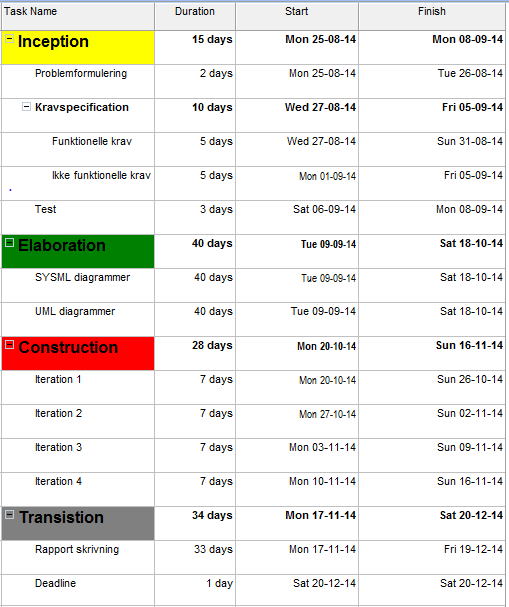
\includegraphics[width=0.6\textwidth]{Billeder/Tidsplan.png}
\caption{Tidsplan}
\label{fig:Tidsplan}
\end{figure}

\newpage

\begin{figure}[V]
\centering
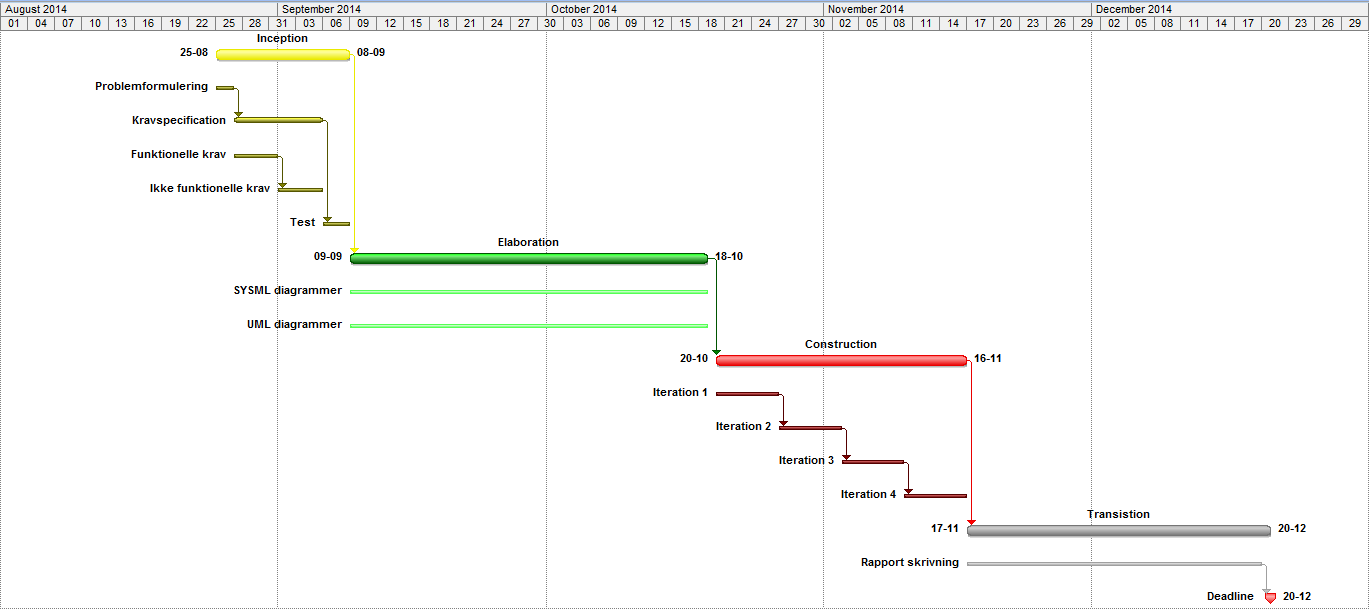
\includegraphics[width=0.7\textwidth]{Billeder/Tidsplan1.png}
\caption{Grafisk tidsplan}
\label{fig:Grafisk_tidsplan}
\end{figure}